\section{Lernfeld 1A - Betrieb und sein Umfeld}

\subsection{tl;dr - Zusammenfassung der Zusammenfassung}
%%% Ende: tl;dr

\subsection{Einführung}
Im Lernfeld 1A \ql Betrieb und sein Umfeld\qr\ werden sowohl Aspekte der Volkswirtschaftslehre (VWL) als auch Betriebswirtschaftslehre (BWL) besprochen. Dabei handelt es sich im Groben um die marko- und mirkoökonomischen Aspekte des wirtschaftlichen Handelns.

In der VWL werden Indikatoren behandelt, welche dazu dienen sollen, die gesamtwirtschaftliche Leistung eines Landes zu messen. Im Kontrast dazu behandelt die BWL Indikatoren zur Bestimmung der Leistung einzelner Unternehmen.

Privatwirtschaftliche Akteure können verschiedene Ziele haben, beispielsweise Gewinnmaximierung oder Gewinnung von Marktanteilen. Öffentliche Akteure stellen in erster Linie Infrastruktur bereit, wie zum Beispiel das Straßenverkehrsnetz.

Allgemein ist wirtschaftendes Handeln notwendig, da die Ressourcen auf unserer Erde begrenzt sind. Dabei gibt es zwei hervorstechende Prinzipien: erstens das {\bf Minimal-Prinzip} und zweitens das {\bf Maximal-Prinzip}. Dem Minimal-Prinzip folgend wird versucht ein festes Ziel mit möglichst wenig Ressourceneinsatz zu erreichen. Beim Maximal-Prinzip wird versucht mit einer festen Menge von Ressourcen ein möglichst großes Ziel zu erreichen.

Warum müssen wir überhaupt wirtschaften? Wir müssen wirtschaften, weil wir Bedürfnisse haben. Die Darstellung von Bedürfnissen erfolgt meist in der Form einer Pyramide. Die wohl bekannteste dieser Darstellung ist die Maslowsche Bedürfnishierarchie.

Produktionsfaktoren sind 

%%% Marktstruktur und Auswirkungen
% Angebot und Nachfrage, Marktarten, Preisbildung, Preiseingriffe d. Staates:

Außerdem werden im Lernfeld die Themen Marktstruktur und ihre Auswirkungen auf das Handeln der Marktteilnehmer besprochen. Grob gesprochen gibt es zwei Arten von Märkten: zum einen den {\bf Käufermarkt} und zum anderen den {\bf Verkäufermarkt}. Auf dem Käufermarkt sind die Käufer im Vorteil, weil es beispielsweise mehr Angebot als Nachfrage gibt. Auf einem Verkäufermarkt sind die oder der Verkäufer im Vorteil, da diese oder dieser ein Monopol durch Patente auf ein gefragtes Produkt hält und so ein geringes Angebot mit hoher Nachfrage besteht.

Durch Angebot und Nachfrage wird der Preis eines Produktes bestimmt. Die folgende Grafik beschreibt die Entstehung des Gleichgewichtspreis.

%%% Anfang: Bild > Gleichgewichtspreis
\begin{wrapfigure}{l}{0.3\textwidth}
	\begin{center}
		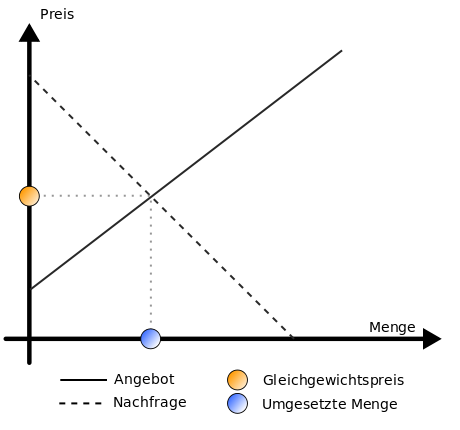
\includegraphics[width=0.28\textwidth]{pictures/lf01-pic/lf01-gleichgewichtspreis.png}
	\end{center}
	\caption{Entstehung des Gleichgewichtspreis}
\end{wrapfigure}
%%% Ende: Bild

Die Angebotslinie startet mit kleinem Angebot bei einem niedrigen Minimalpreis und wächst mit steigendem Preis. Die Nachfragelinie startet mit einer kleinen Nachfrage bei einem hohen Maximalpreis und nimmt mit fallendem Preis immer weiter an Menge zu. Wie an diesen zwei Linien zu erkennen ist, gibt es immer mehr Anbieter und Ware je höher der verlangte Preis ist. Umgekehrt gibt es immer mehr Abnehmer, die immer mehr kaufen, je niedriger der für die Ware verlangte Preis ist. Da die Preiswünsche von Anbietern und Abnehmern gegenläufig sind, stellt sich im Markt ein Gleichgewicht an der Schnittstelle von Angebot und Nachfrage ein, die den Gleichgewichtspreis und das Maximum des Umsatzes festlegt.

Marktsättigung führt dazu, dass kontinuierlich neue Produkte entwickelt werden müssen. Ein hilfreiches Instrument, um eine dauerhafte Marktsättigung zu umgehen, ist die geplante Obsoleszenz. Es werden absichtlich Bauteile verwendet, die nur eine begrenzte Lebenszeit haben; idealerweise beträgt die Lebenszeit eines solchen Bauteils nicht länger als die gesetzlich vorgeschriebene Garantiezeit. Dadurch wird eine konstante Nachfrage generiert.

%%% Ende: Einführung
%%%%%%%%%%%%%%%%%%%%%%%%%%%%%%%%%%%%%%%%%%%%%%%%%%%%%%%%%%%%%%%%%%%%%%%%%%%%%%%%

%%% Anfang: Werbung
\subsection{Werbung}

Was versteht das Recht unter sogenannten \ql Lockangeboten\qr? Welche Art von Werbung ist erlaubt und welche nicht? Diese und weitere Fragen werden in diesem Abschnitt beantwortet.

Für beworbene Waren gilt eine Vorratsfrist von zwei Tagen. In Ausnahmen darf diese auch weniger getragen, beispielsweise wenn die Höhe der Nachfrage nicht absehbar war. Die Formulierung \ql Solange der Vorrat reicht\qr\ hebelt die Vorratsfrist aus, aber nur falls keine Vorerfahrung über die Höhe der Nachfrage bestand.

Das Gesetz gegen unlauteren Wettbewerb (UWG) regelt, welche Formen der Werbung erlaubt sind und unter welchen Umständen sie als unlauter gelten.

Der Zweck von Lockangeboten besteht darin, Kunden in den Laden zu locken. Diese kommen bereits mit einer Kaufabsicht in den Laden. Wenn dann das beworbene Angebot nicht mehr erhältlich ist, greifen viele dieser Kunden zu einem ähnlichen aber teureren Produkt. 

Vergleichende Werbung ist nur in wenigen Fällen unproblematisch, sodass meistens darauf verzichtet wird.

Unter \ql Mondpreiswerbung\qr\ wird eine künstliche Erhöhung des Preises verstanden, um anschließend mit einer Reduzierung des Preises zu werden. Preise müssen normalerweise 6 Monate lang konstant bleiben.

Außerdem fällt unzumutbare Belästigung in den Bereich des unlauteren Wettbewerbs.

Im Einzelnen wurden die Paragraphen 3 bis 7 des UWG besprochen. Die Überschriften der Paragraphen lauten:
\begin{itemize}
	\item[§3] Verbot unlauterer geschäftlicher Handlungen
			\begin{itemize}
				\item Interessen von Mitbewerbern, Verbrauchern oder sonstigen Marktteilnehmern dürfen nicht spürbar beeinträchtigt werden.
				\item Geschäftliche Handlungen gegenüber Verbrauchern sind unzulässig, wenn sie nicht der für den Unternehmer geltenden fachlichen Sorgfalt entsprechen.
				\item Die Fähigkeit des Verbrauchers, sich auf Grund von Informationen zu entscheiden, darf nicht spürbar beeinträchtigt werden. Er darf nicht zu einer geschäftlichen Entscheidung veranlasst werden, die er sonst nicht getroffen hätte.
			\end{itemize}
	\item[§4] Beispiele unlauterer geschäftlicher Handlungen
			\begin{enumerate}
				\item Entscheidungsfreiheit der Marktteilnehmer durch Ausübung von Druck, in menschenverachtender Weise oder durch sonstigen unangemessenen unsachlichen Einfluss zu beeinträchtigen.
				\item Ausnutzen von geistigen oder körperlichen Gebrechen, des Alters, der geschäftlichen Unerfahrenheit, der Leichtgläubigkeit, der Angst oder der Zwangslage des Marktteilnehmers
				\item Verschleierung des Werbecharakters geschäftlicher Handlungen
				\item Bedingungen für die Inanspruchname von Verkaufsförderungsmaßnahmen wie Preisnachlässen, Zugaben oder Geschenken werden nicht klar und eindeutig angegeben
				\item Teilnahmebedingungen werden bei Preisausschreiben oder Gewinnspielen mit Werbecharakter nicht klar und eindeutig angegeben
				\item Teilnahme von Verbrauchern an einem Preisausschreiben oder einem Gewinnspiel ist an den Erwerb einer Ware oder die Inanspruchname einer Dienstleistung abhängig. \\
{\it Ausnahme:} Das Preisausschreiben oder Gewinnspiel ist naturgemäß mit der Ware oder Dienstleistung verbunden
				\item Die Kennzeichen, Waren, Dienstleistungen, Tätigkeiten oder persönlichen geschäftlichen Verhältnisse eines Mitbewerbers werden herabgesetzt oder verunglimpft			
				\item über die Waren, Dienstleistungen oder das Unternehmen eines Mitbewerbers oder über Unternehmer oder ein Mitglied der Unternehmensleitung Tatsachen behaupten oder verbreiten, die geeignet sind, den Betrieb des Unternehmens oder den Kredit des Unternehmers zu schädigen, sofern die Tatsachen nicht erweislich wahr sind.
			\end{enumerate}
	\item[§5] Irreführende geschäftliche Handlungen
		\begin{itemize}
			\item Eine geschäftliche Handlung ist Irreführend, wenn sie unwahre Angaben enthält oder sonstige zur Täuschung geeigneten Angaben über die wesentlichen Merkmale der Ware oder Dienstleistung oder den Anlass des Verkaufs enthält
			\item Verwechslungsgefahr mit einer anderen Ware oder Dienstleistung oder mit der Marke oder einem anderen Kennzeichen eines Mitbewerbers wird hervorgerufen
			\item Werbung mit einer Herabsetzung eines Preises, sofern der Preis nur eine unangemessen kurze Zeit gefordert worden ist ({\it Mondpreiswerbung})
		\end{itemize}
	\item[§5a] Irreführung durch Unterlassung
		\begin{itemize}
			\item Beeinflussung der Entscheidungsfähigkeit der Marktteilnehmer durch verschweigen wesentlicher Informationen
		\end{itemize}
	\item[§6] Vergleichende Werbung
		\begin{itemize}
			\item Vergleich bezieht sich nicht auf Waren oder Dienstleistungen für den gleichen Bedarf oder dieselbe Zweckbestimmung
			\item Nicht objektive auf wesentliche, relevante, nachprüfbare und typische Eigenschaften oder den Preis bezogen ist
			\item Verwechslung mit Mitbewerbern oder von diesen angebotenen Produkten
			\item Ruf des von einem Mitbewerber verwendeten Kennzeichen wird in unlauterer Weise ausgenutzt oder beeinträchtigt
			\item Ware oder Dienstleistung als Imitation oder Nachahmung einer unter einem geschützten Kennzeichen vertriebenen Ware oder Dienstleistung darstellen
		\end{itemize}
	\item[§7] Unzumutbare Belästigung
		\begin{itemize}
			\item Werbung, obwohl erkennbar ist, dass der angesprochene Marktteilnehmer diese Werbung nicht wünscht
			\item Werbung mit einem Telefonanruf gegenüber einem Verbraucher ohne dessen vorherige ausdrückliche Einwilligung
			\item Werbung unter Verwendung einer automatischen Anrufmaschine, eines Faxgeräts oder elektronischer Post, ohne vorherige ausdrückliche Einwilligung des Adressaten
			\item Verschleierung der Identität des Absenders
		\end{itemize}
\end{itemize}

%%% Ende: Werbung
%%%%%%%%%%%%%%%%%%%%%%%%%%%%%%%%%%%%%%%%%%%%%%%%%%%%%%%%%%%%%%%%%%%%%%%%%%%%%%%%

%%% Anfang: Betriebliche Kennzahlen
\subsection{Betriebliche Kennzahlen}

Als Kennziffern werden Indikatoren zur Bestimmung des wirtschaftlichen Erfolges bezeichnet, welche in Form von Zahlen ermittelt werden können. Dazu gehören offensichtliche Werte wie der Gewinn eines Unternehmens als auch die Produktivität. Betriebliche Kennzahlen können unter anderem in Relation zum Vorjahr, der Auslastung oder der Konkurrenz betrachtet werden.\\

%%% Formeln zur Berechnung der Kennziffern:

% Produktivität
Die Produktivität ist eine {\bf Messgröße für die Ergiebigkeit der in der Produktion eingesetzten Produktionsfaktoren}. \\
$Produktivität = \frac{mengenmäßige Ausbringungsmenge}{mengenmäßigen Einsatz der Produktionsfaktoren} = \frac{Output}{Input}$\\
$Arbeitsproduktivität = \frac{mengenmäßige Ausbringungsmenge}{Arbeitsstunden}$\\
\\
% Wirtschaftlichkeit
Bei der Berechnung der Wirtschaftlichkeit handelt es sich um eine Erweiterung der Produktivität um den Faktor Geld. Zur Berechnung der Wirtschaftlichkeit werden die wertmäßigen Leistungen auf den Wert der eingesetzten Produktionsfaktoren bezogen.\\
$Wirtschaftlichkeit = \frac{Leistungen}{Kosten}$\\
\\
% Produktivitätsfaktor
% Rentabilität
Die Erzielung von Gewinnen ist das Ziel privatwirtschaftlicher Unternehmen. Zur Beurteilung des Erfolges muss der Gewinn in Bezug zum eingesetzten Kapital gesetzt werden.\\
$Eigenkapitalrentabilität = \frac{Gewinn \times 100}{Eigenkapital}$\\
\\
Die Gesamtkapitalrentabilität zeigt an, wie sich das gesamte in der Unternehmung eingesetzte Kapital verzinst. Zur Erzielung von Gewinn aus dem eingesetzten Fremdkapital muss die Eigenkapitalrentabilität über dem Fremdkapitalzins liegen.\\
$Gesamtkapitalrentabilität = \frac{(Gewinn + Fremdkapital) * 100}{Eigenkapitel + Fremdkapital}$\\
\\
% Bilanzanalyse
% Investitionsanalyse
% Quoten
Die Eigenkapitalquote setzt das Eigenkapital in Bezug zum Gesamtkapital des Unternehmens.\\
$Eigenkapitalquote = \frac{Eigenkapital * 100}{Gesamtkapital}$\\
\\
Die Fremdkapitalquote setzt das eingebrachte Fremdkapital in Bezug zum Gesamtkapital des Unternehmens.\\
$Fremdkapitalquote = \frac{Fremdkapital * 100}{Gesantkapital}$\\
\\
Der Verschuldungsgrad gibt den Anteil des Fremdkapitals am Eigenkapital an.\\
$Verschuldungsgrad = \frac{Fremdkapital * 100}{Eigenkapital}$\\
\\
% Intensitäten
Die Anlageintensität gibt den Anteil des Anlagevermögens (dem Unternehmen dauerhaft dienend) am Gesamtvermögen an.\\
$Anlageintensität = \frac{Anlagevermögen * 100}{Gesamtvermögen}$\\
\\
Die Arbeitsintensität gibt den Anteil des Umlaufvermögens (dem Unternehmen kurzzeitig dienend, z.B. auf Lager liegende Waren) am Gesamtvermögen an.\\
$Arbeitsintensität = \frac{Umlaufvermögen * 100}{Gesamtvermögen}$\\
\\
% Finanzierungsanalyse
% Liquiditätsanalyse
Der Anlagendeckungsgrad I gibt an, welcher Anteil des Anlagevermögens durch Eigenkapital gedeckt ist. Nach der {\it Goldenen Bilanzregel im engeren Sinne} sollte das Anlagevermögen durch Eigenkapital finanziert werden.\\
$Anlagedeckungsgrad I = \frac{Eigenkapital}{Anlagevermögen}$\\
\\
Der Anlagendeckungsgrad II gibt an, welcher Anteil des Anlagevermögens durch Eigenkapital und langfristiges Fremdkapital gedeckt ist. Nach der {\it Goldenen Bilanzregel im weiteren Sinne} soll die Finanzierung durch langfristig zur Verfügung stehendes erfolgen.\\
$Anlagedeckungsgrad II = \frac{Eigenkapital + langfristiges Fremdkapital}{Analgevermögen}$\\
\\
%Liquidität
Die Liquidität ist eine Existenzbedingung des Unternehmens, die auch kurzfristig immer gesichert sein muss, um eine Zahlungsfähigkeit zu gewährleisten und eine eventuelle Gefahr für den Fortbestand durch Zahlungsunfähigkeit zu verhindern.\\
Flüssige Mittel = Kasse, Postgiroguthaben, Guthaben bei Kreditinstituten, Schecks, diskontfähige Wechsel und börsengängige Wertpapiere\\
Kurzfristige Forderungen = Forderungen mit einer Restlaufzeit bis zu einem Jahr\\
Kurzfristige Verbindlichkeiten = Verbindlichkeiten mit einer Restlaufzeit bis zu einem Jahr\\

$Liquidität 1. Grades = \frac{Flüssige Mittel * 100}{Kurzfristige Verbindlichkeiten}$\\
$Liquidität 2. Grades = \frac{(Flüssige Mittel + kurzfr. Forderungen) * 100}{Kurzfristige Verbindlichkeiten}$\\
$Liquidität 3. Grades = \frac{Umlaufvermögen * 100}{Kurzfristige Verbindlichkeiten}$\\

%%% Ende: Betriebliche Kennzahlen
%%%%%%%%%%%%%%%%%%%%%%%%%%%%%%%%%%%%%%%%%%%%%%%%%%%%%%%%%%%%%%%%%%%%%%%%%%%%%%%%

%%% Anfang: Wirtschaftskreislauf
\subsection{Wirtschaftskreislauf}

Der Wirtschaftskreislauf beschreibt den Austausch von Gütern, Dienstleistungen und Geld. Dadurch werden die Zusammenhänge der einzelnen Akteure (Unternehmen, Haushalte, Banken, Staaten \dots) deutlich.

Manchmal werden Preise mit negativem Deckungsbeitrag -- das sind Preise, die unter den Produktionskosten liegen -- ausgeschrieben, um beispielsweise eine stärkere Marktdurchdringung oder eine Verdrängung von Konkurrenz zu erreichen. Ein negativer Deckungsbeitrag wird auch verwendet, um seine Lagerbestände zu leeren. \\
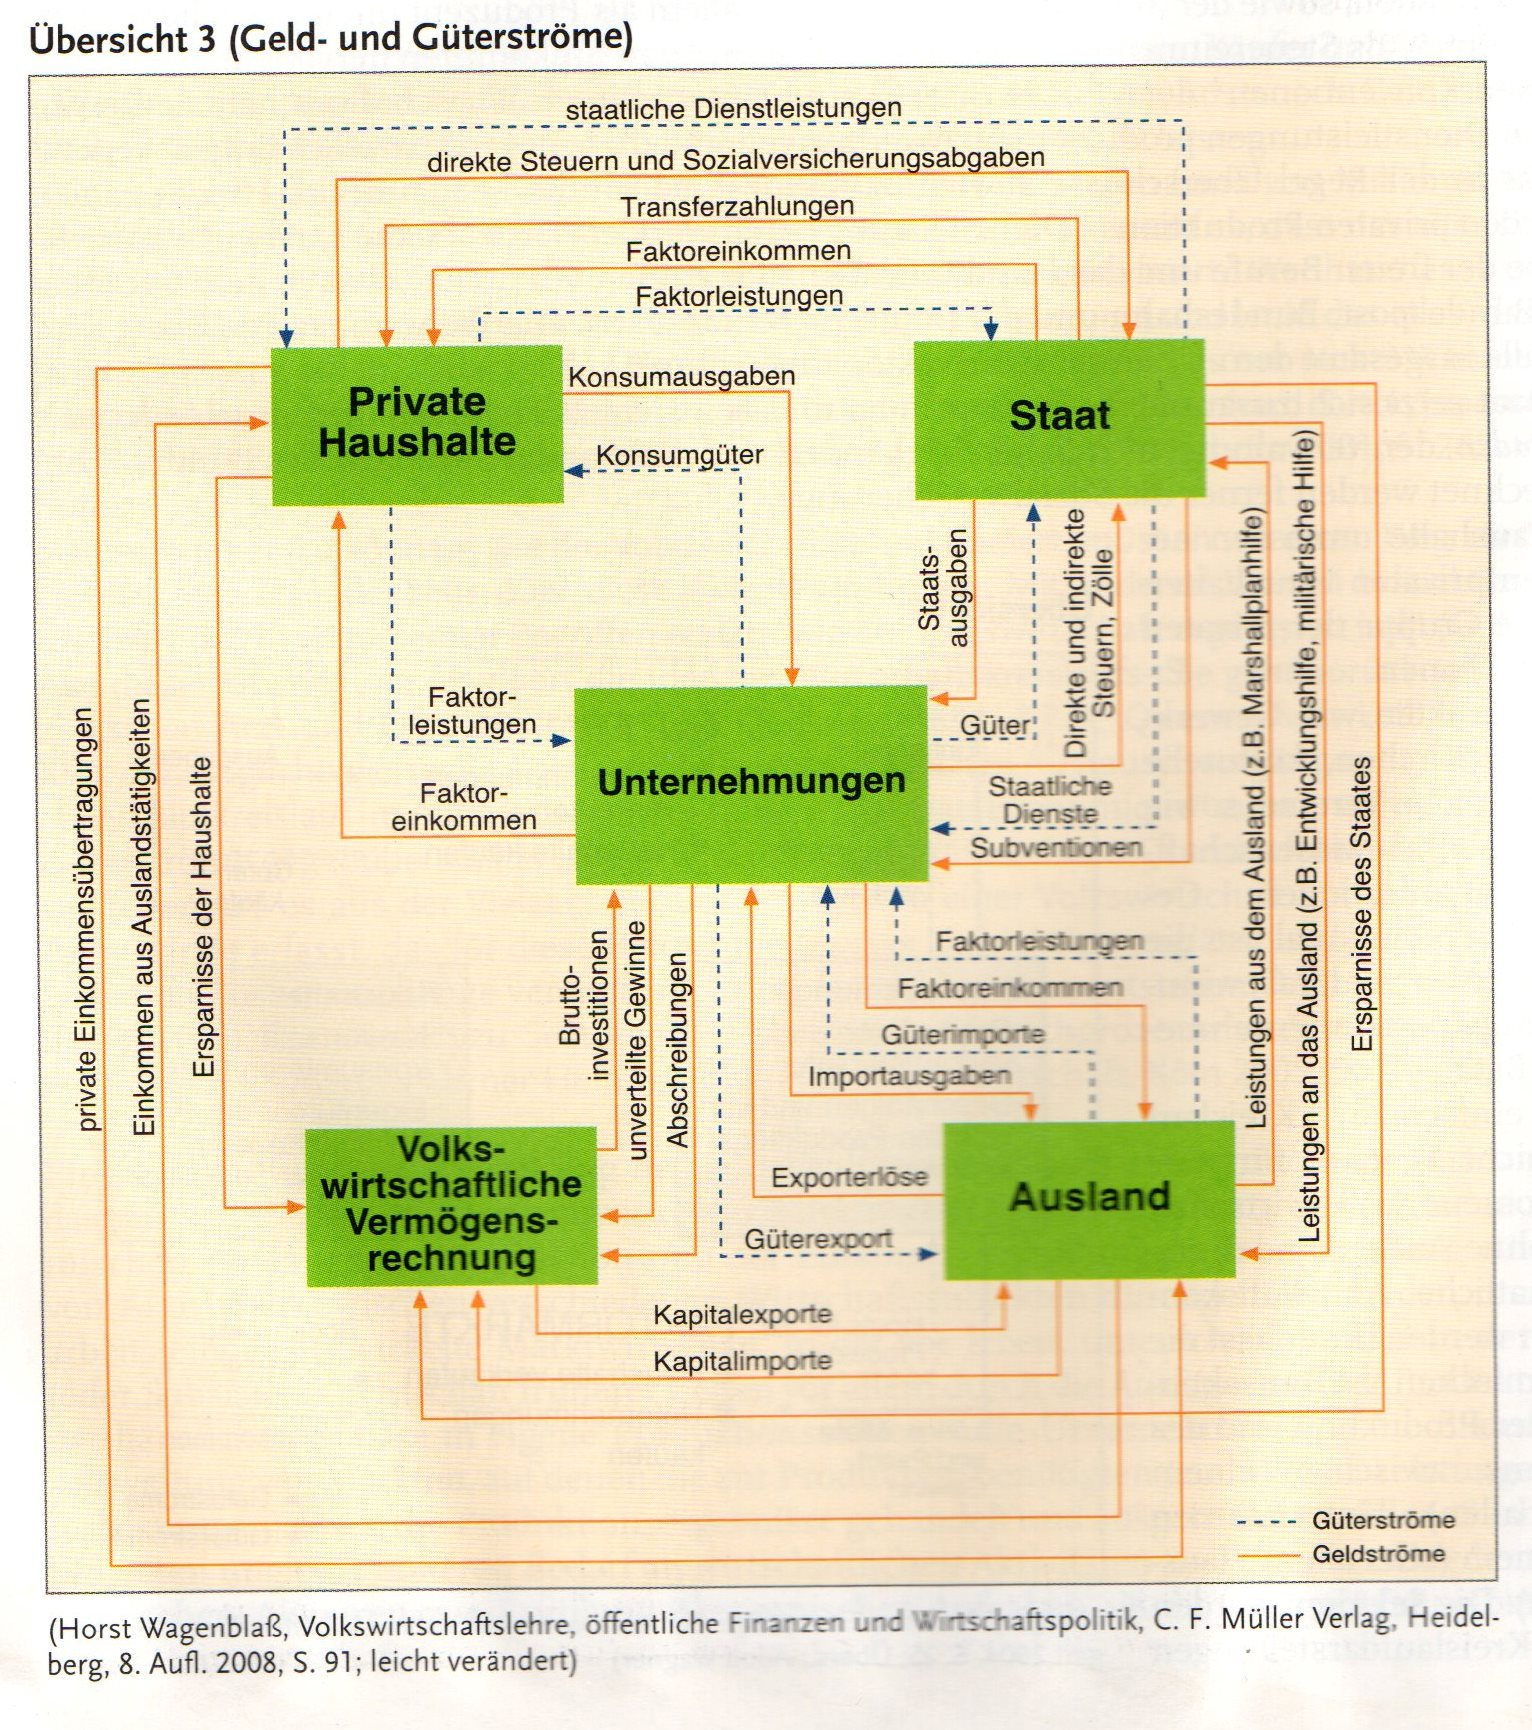
\includegraphics[scale=1.0]{pictures/lf01-pic/lf01-wirtschaftskreislauf.jpg}

%%% Ende: Wirtschaftskreislauf
%%%%%%%%%%%%%%%%%%%%%%%%%%%%%%%%%%%%%%%%%%%%%%%%%%%%%%%%%%%%%%%%%%%%%%%%%%%%%%%%

%%% Anfang: Marktstrukturen und ihre Auswirkungen
\subsection{Marktstrukturen und ihre Auswirkungen}

Was ist ein Markt? Märkte sind Orte, an denen Angebot und Nachfrage aufeinandertreffen und durch den Ausgleich von Angebot und Nachfrage bildet sich ein Preis. Es gibt verschiedene Arten von Märkten, zum einen Faktormärkte -- bspw. Arbeitsmarkt -- und zum anderen Gütermärkte. Daneben gibt es noch verschieden Marktformen:\\
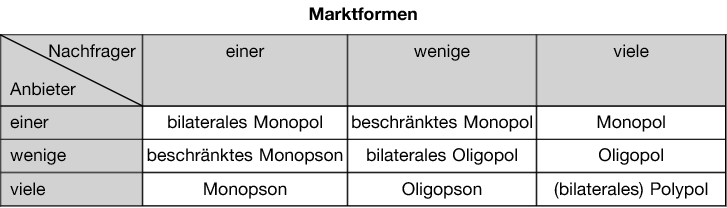
\includegraphics[scale=0.6]{pictures/lf01-pic/lf01-marktformen.png}

\subsubsection{Anbieter- und Nachfragerverhalten}
Das Verhalten von Anbietern und Nachfragern stellen Einflussfaktoren auf den Märkten dar.

{\bf Einflussfaktoren auf Seiten der Anbieter:}
\begin{itemize}
	\item Kosten der Produktionsfaktoren
	\item Gewinnerwartung
	\item Preis des Angebots
	\item Preis der Konkurrenz
	\item Stand der technischen Entwicklung
\end{itemize}

{\bf Einflussfaktoren auf Seiten der Nachfrager: }
\begin{itemize}
	\item Art und Dringlichkeit der Nachfrage
	\item Preis des nachfragten Gutes
	\item Preise der Konkurrenz
	\item Höhe der Kaufkraft
	\item Zukunftserwartungen der Konsumenten
\end{itemize}

Bei dem vollkommenen Markt handelt es sich um eine theoretische Vereinfachung der Realität. Der vollkommene Markt erfüllt folgende Bedingungen:

\begin{itemize}
	\item Rationales Verhalten aller Teilnehmer
	\item Homogenität aller Güter
	\item Keine Präferenzen der Teilnehmer
	\item Vollständige Markttransparenz
	\item Unendliche Reaktionsgeschwindigkeit der Teilnehmer
\end{itemize}

Durch diese Optimalisierung der Realität gibt es nahezu nur unvollkommene Märkte. Dem vollkommenen Markt am nächsten kommt die Börse. \\

Unter den Annahmen, dass vollständige Konkurrenz herrscht und dass Angebot und Nachfrage bloß vom Preis abhängen, gilt: (1) Wenn der Preis steigt, sinkt die Nachfrage \& (2) Wenn der Preis steigt, dann steigt das Angebot.\\

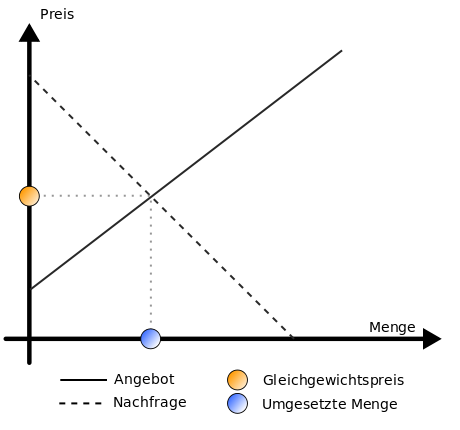
\includegraphics[scale=0.7]{pictures/lf01-pic/lf01-gleichgewichtspreis.png}\\
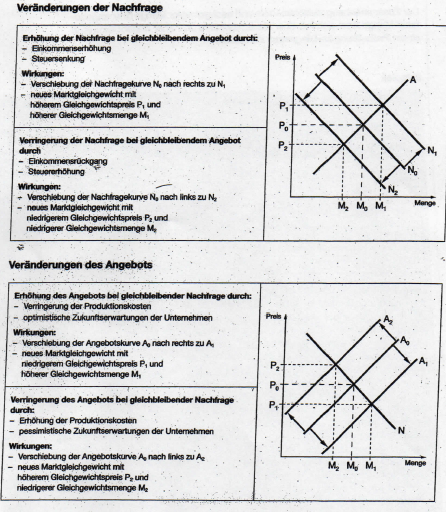
\includegraphics[scale=1.0]{pictures/lf01-pic/lf01-nachfrageverschiebung.png}
%%% Ende: Marktsturkturen und ihre Auswirkungen
%%%%%%%%%%%%%%%%%%%%%%%%%%%%%%%%%%%%%%%%%%%%%%%%%%%%%%%%%%%%%%%%%%%%%%%%%%%%%%%%

%%% Anfang: Kooperation \& Konzentration
\subsection{Kooperation \& Konzentration}

\begin{itemize}
	\item horizontale Kooperation
		\begin{itemize}
			\item Unternehmen gleicher Wirtschaftsstufe
			\item gleichartige Güter werden produziert
		\end{itemize}
	\item vertikale Kooperation
		\begin{itemize}
			\item Unternehmen unterschiedlicher Wirtschaftsstufen
		\end{itemize}
	\item anorganische Kooperation
		\begin{itemize}
			\item Unternehmen unterschiedlicher Wirtschaftsstufen und Branchen
		\end{itemize}
\end{itemize}

\begin{itemize}
	\item horizontale Konzentration
		\begin{itemize}
			\item Unternehmen gleicher Wirtschaftsstufe und Branche fusionieren zu einem Unternehmen
		\end{itemize}
	\item vertikale Konzentration
		\begin{itemize}
			\item Unternehmen unterschiedlicher Wirtschaftsstufen und gleicher Branche fusionieren zu einem Unternehmen
			\item Ein größerer Teil der Produktionskette kann von dem neuen Unternehemen verwirklicht werden
		\end{itemize}
	\item diagonale Konzentration
		\begin{itemize}
			\item Unternehmen unterschiedlicher Wirtschaftsstufen und Branchen fusionieren zu einem Unternehmen
			\item Ein Mischkonzern entsteht
			\item Es wird für Risikosträuung gesorgt
		\end{itemize}
\end{itemize}


\subsection{Entgeltabrechnung}

\subsubsection{Gehaltsbestandteile} 
Das Gehalt kann sich aus mehreren Faktoren zusammensetzen:
\begin{itemize}
	\item Grundlohn
	\item Naturallohn
		\begin{itemize}
			\item z.B. zusätzlich bei der Seeschiffahrt, im Nahrungsmittelbereich als "freie Kost und Logis"
		\end{itemize}
	\item Zeitlohn
		\begin{itemize}
			\item Bezahlung auf Basis der geleisteten Arbeitszeit
		\end{itemize}
	\item Zuschlag
		\begin{itemize}
			\item Zuschläge für besondere Leistungen oder Belastungen des Arbeitsnehmers
			\item z.B. überstunden, Nachtarbeit, Spätschicht, Schmutzzuschlag, Hitzezuschlag, Kinderzuschlag, Ortszuschlag, Leistungszuschlag
		\end{itemize}
	\item Akkordlohn
		\begin{itemize}
			\item Bezahlung nach geleistetem Arbeitsergebnis unabhängig von der Arbeitszeit
		\end{itemize}
	\item Prämiensystem
		\begin{itemize}
			\item Zeitlohn und zusätzlich entsprechend der Leistung eine Prämie
		\end{itemize}
	\item Provision
		\begin{itemize}
			 \item Prozentuale Beteiligung am Wert der eigenen Geschäfte
		\end{itemize}
	\item Gratifikation
		\begin{itemize}
			\item Sonderzuwendung bei besonderen Anlässen
			\item z.B. Weihnachten, Jubiläum, Erreichung eines besonderen Ziels
		\end{itemize}
	\item Gewinnbeteiligung
		\begin{itemize}
			\item Beteiligung am Geschätsergebnis des Unternehmens
		\end{itemize}
	\item Vermögenswirksame Leistungen
		\begin{itemize}
			\item Ein Teil des Arbeitsverdienstes wird vermögenswirksam angelegt
			\item Arbeitgeber kann sich durch individuelle Vereinbarungen an den Beiträgen beteiligen
		\end{itemize}
	\item Aufwendungsersatz
		\begin{itemize}
			\item Aufwendungen des Arbeitnehmers müssen ersetzt werden
			\item z.B. Reisespesen oder Auslagen zur Beschaffung von Werkzeugen
		\end{itemize}
\end{itemize}

\subsubsection{Abzüge}
Faktoren, die sich auf die Gehaltsabrechnung auswirken:
\begin{itemize}
	\item Einkommenshöhe
		\begin{itemize}
			\item Die Lohnsteuer wird nur auf den Einkommensanteil oberhalb des Grundfreibetrages erhoben
		\end{itemize}
	\item Familienstand: Steuerklasse
	\item Kirchenmitgliedschaft
		\begin{itemize}
			\item Kirchensteuer
		\end{itemize}
	\item Krankenkasse
		\begin{itemize}
			\item Variable Zusatzbeiträge
		\end{itemize}
	\item Wohnort
		\begin{itemize}
			\item Solidaritätszuschlag
			\item Kirchensteuersatz
		\end{itemize}
\end{itemize}

Die Beiträge zur Sozialversicherung werden zur Hälfte vom Arbeitgeber getragen:
\begin{itemize}
	\item Rentenversicherung (19,9\%)
	\item Pflegeversicherung (1,7\% + 0,25\% für Kinderlose ab einem Alter von 23 Jahren)
	\item Arbeitslosigkeit (4,2\%)
	\item Krankenkasse (variabel + 0,9\% Zusatzbeitrag für Arbeitnehmer)
\end{itemize}
Bei Azubis mit einem Gehalt unter 325\euro brutto übernimmt der Arbeitgeber die Versicherungsbeiträge vollständig.

Weiter Abzüge: Lohnsteuer, Solidaritätsbeitrag, Kirchensteuer

Lohnsteuerklassen:
\begin{itemize}
	\item Klasse I: ledig, geschieden, verwitwet
	\item Klasse II: Steuerklasse I mit min. einem Kind
	\item Klasse III: verheiratet, ein Verdiener
	\item Klasse IV: verheiratet, zwei Verdiener in IV, beide Verdienen etwa gleich viel
	\item Klasse V: verheiratet, zwei Verdiener, Partner in III, Verdienst ist unterschiedlich
	\item Klasse VI: mehrere Lohnsteuerkarten
\end{itemize}

\subsubsection{Beispielabrechnung}
Voraussetzungen: Angestellte, ledig, 24 Jahre, 2.100\euro brutto, Lohnsteuer: 287,33\euro , Kirchensteuersatz 9\%, Solidaritätszuschlag: 5,5\% Beitragssatz zur Krankenkasse: allgemeiner Beitragssatz: 13,8\%, zusätzlicher Beitragssatz: 0,9\%, Beitragssatz zur Rentenversicherung: 19,5\%
Beitragssatz zur Arbeitslosenversicherung: 4,5\%, Beitragssatz zur Pflegeversicherung: 1,7\% \\
\\
$Kirchensteuer = Lohnsteuer * Kirchensteuersatz = 287,33\textit{\euro} * 9\% = 25,85\textit{\euro}$\\
$Solidaritätszuschlag = Lohnsteuer * 5,5\% = 287,33\textit{\euro} * 5,5\% = 15,80\textbf{\euro}$\\
$Krankenversicherung = \frac{Bruttolohn * Krankenversicherungssatz}{2} + Bruttolohn * Zusatzbeitrag = \frac{2100\textit{\euro} * 13,8\%}{2}+2100\textit{\euro} * 9\% = 163,80\textit{\euro}$\\
$Rentenversicherung = \frac{Bruttolohn * Rentenversicherungssatz}{2} = \frac{2100\textit{\euro}}{2} = 204,75\textit{\euro}$\\
$Arbeitslosenversicherung = \frac{Bruttolohn * Arbeitslosenversicherungssatz}{2} = \frac{2100\textit{\euro}* 4,5\%}{2} = 47,25\textit{\euro}$\\
$Pflegeversicherung = \frac{Bruttolohn * Pflegeversicherungssatz}{2} + Bruttolohn * Zusatzbeitrag = \frac{2100\textit{\euro} * 1,7\%}{2} + 2100\textit{\euro} * 0,25\% = 23,10\textit{\euro}$\\
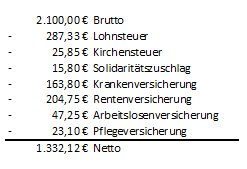
\includegraphics[scale=1.0]{pictures/lf01-pic/lf01-beispielentgeldabrechung.png}


\subsection{Rechts- und Geschäftsfähigkeit}

Wichtige Punkte, die in einem Kaufvertrag notiert werden sollten:
\begin{itemize}
	\item Art und Güte der Leistung
	\item Lieferzeit
	\item Verpackungs- und Versandkosten
	\item Zahlungsart
	\item Preis
	\item Erfüllungsort
\end{itemize}

\subsubsection{Rechtsordnung}
Die Rechtsordnung unterscheidet zwischen dem öffentlichen und dem Privaten Recht.\\
Das {\it öffentliche Recht} beschreibt die Rechtsbeziehungen zwischen den Einzelpersonen und dem Staat. Dies ist z. B. im Steuerrecht und im Strafrecht der Fall.\\
Das {\it Private Recht} beschreibt die Rechtsbeziehungen zwischen den Einzelpersonen, wie es z. B. im BGB und im HGB der Fall ist.\\
\\
\begin{itemize}
	\item Rechtsfähigkeit
		\begin{itemize}
			\item Fähigkeit, Träger von Rechten und Pflichten zu sein
			\item Natürliche Personen
				\begin{itemize}
					\item Menschen von Geburt bis Tod
				\end{itemize}
			\item Juristische Personen
				\begin{itemize}
					\item Vereine
					\item Stiftungen
					\item Handelsgesellschaften mit Eintragung in das jeweilige Register (z.B. GmbH, AG)
				\end{itemize}
		\end{itemize}
	\item Geschäftsfähigkeit
		\begin{itemize}
			\item Fähigkeit, selbstständig und wirksam Rechtsgeschäfte abschließen zu können
			\item geschäftsunfähig (Willenserklärungen sind nichtig)
				\begin{itemize}
					\item Kinder bis zum vollendeten 7. Lebensjahr
					\item geschäftsunfähige Personen (§ 104 BGB)
					\item {\it Ausnahmen:} volljährige Geschäftsunfähige, die Geschäfte des täglichen Lebens mit geringen Mitteln bewirken (§ 105 BGB)
				\end{itemize}
			\item beschränkt geschäftsfähig (Willenserklärungen sind schwebend unwirksam)
				\begin{itemize}
					\item Kinder zwischen dem vollendeten 7. und vollendetem 18. Lebensjahr (§§ 106 bis 113 BGB)
					\item betreute Volljährige mit gerichtlichem Einwilligungsvorbehalt für bestimmte Handlungsbereiche. {\it Hinweis:} Der gesetzliche Vertreter kann auch nachträglich genehmeigen.
					\item Taschengeldgeschäfte nach § 110 BGB
					\item vorteilhafte Rechtsgeschäfte nach § 107 BGB
					\item selbstständiger Betrieb eines Erwerbsgeschäftes nach § 112 BGB
					\item genehmigte Arbeitsverhältnisse nach § 113 BGB
				\end{itemize}
			\item voll geschäftsfähig 
				\begin{itemize}
					\item alle sonstigen volljährigen Personen
				\end{itemize}
		\end{itemize}
	\item Deliktfähigkeit (vgl. § 828 BGB) / Schuldfähigkeit (vgl. § 19 StGB)
		\begin{itemize}
			\item Verantwortung für unerlaubte Handlungen (Aufsichtspflicht beachten)
		    \item deliktunfähig
		    	\begin{itemize}
		    		\item Kinder bis zur Vollendung des 7. Lebensjahres
		    	\end{itemize}
		    \item beschränkt deliktfähig
		    	\begin{itemize}
		    		\item Minderjährige zwischen 7 und 18 Jahren und Taubstumme (Schuldfähigkeit ab 14 Jahren)
		     	\end{itemize}
		     \item voll deliktfähig
		     	\begin{itemize}
		     		\item Personen ab Vollendung des 18. Lebensjahres, sofern geschäftsfähig
		     	\end{itemize}
		\end{itemize}
	
\end{itemize}
\subsubsection{Rechtsgeschäfte}

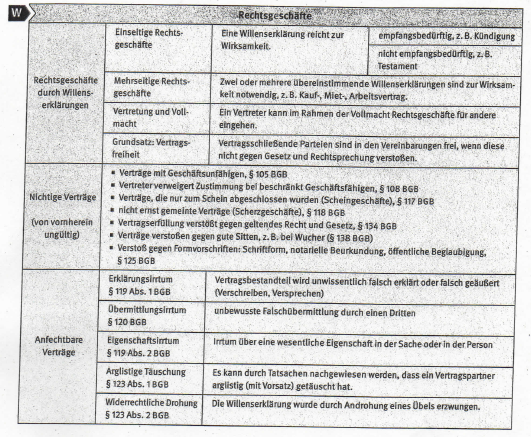
\includegraphics[scale=1.3]{pictures/lf01-pic/lf01-rechtsgeschaefte.png} 

%%% Ende: Entgeltabrechnung
%%%%%%%%%%%%%%%%%%%%%%%%%%%%%%%%%%%%%%%%%%%%%%%%%%%%%%%%%%%%%%%%%%%%%%%%%%%%%%%%